% Capitolul 3: Distribuții stabile ($\alpha$-stabile)
% Statistica Piețelor Financiare
% Program de licență, Academia de Studii Economice din București

\documentclass[9pt, aspectratio=169, t]{beamer}

% Asigură încadrarea conținutului pe diapozitive
\setbeamersize{text margin left=8mm, text margin right=8mm}

%=============================================================================
% CONFIGURARE TEMĂ ȘI STIL
%=============================================================================
\usetheme{default}
% Utilizăm tema implicită pentru control curat al antetului/subsolului

% Paletă de Culori (potrivită cu PDF-ul Redispatch)
\definecolor{MainBlue}{RGB}{26, 58, 110}
\definecolor{AccentBlue}{RGB}{26, 58, 110}
\definecolor{IDAred}{RGB}{205, 0, 0}
\definecolor{DarkGray}{RGB}{51, 51, 51}
\definecolor{MediumGray}{RGB}{128, 128, 128}
\definecolor{LightGray}{RGB}{248, 248, 248}
\definecolor{VeryLightGray}{RGB}{235, 235, 235}
\definecolor{KeynoteGray}{RGB}{218, 218, 218}
\definecolor{SectionGray}{RGB}{120, 120, 120}
\definecolor{FooterGray}{RGB}{100, 100, 100}
\definecolor{Crimson}{RGB}{220, 53, 69}
\definecolor{Forest}{RGB}{46, 125, 50}
\definecolor{Amber}{RGB}{181, 133, 63}
\definecolor{Orange}{RGB}{230, 126, 34}
\definecolor{Purple}{RGB}{142, 68, 173}

% Fundal gradient (gradient Keynote exact 315°: alb la RGB 218,218,218)
\setbeamertemplate{background}{%
    \begin{tikzpicture}[remember picture, overlay]
        \shade[shading=axis, shading angle=315,
        top color=white, bottom color=KeynoteGray]
        (current page.south west) rectangle (current page.north east);
    \end{tikzpicture}%
}
% Culoare solidă de rezervă pentru compatibilitate
\setbeamercolor{background canvas}{bg=}

\setbeamercolor{palette primary}{bg=MainBlue, fg=white}
\setbeamercolor{palette secondary}{bg=MainBlue!85, fg=white}
\setbeamercolor{palette tertiary}{bg=MainBlue!70, fg=white}
\setbeamercolor{structure}{fg=MainBlue}
\setbeamercolor{title}{fg=IDAred}
\setbeamercolor{frametitle}{fg=IDAred, bg=}
\setbeamercolor{block title}{bg=MainBlue, fg=white}
\setbeamercolor{block body}{bg=VeryLightGray, fg=DarkGray}
\setbeamercolor{block title alerted}{bg=Crimson, fg=white}
\setbeamercolor{block body alerted}{bg=Crimson!8, fg=DarkGray}
\setbeamercolor{block title example}{bg=Forest, fg=white}
\setbeamercolor{block body example}{bg=Forest!8, fg=DarkGray}
\setbeamercolor{item}{fg=MainBlue}

% Culori subsol (suprascriu albastrul temei Madrid)
\setbeamercolor{author in head/foot}{fg=FooterGray, bg=}
\setbeamercolor{title in head/foot}{fg=FooterGray, bg=}
\setbeamercolor{date in head/foot}{fg=FooterGray, bg=}
\setbeamercolor{section in head/foot}{fg=FooterGray, bg=}
\setbeamercolor{subsection in head/foot}{fg=FooterGray, bg=}

% Stiluri marcatori (se aplică peste tot inclusiv în blocuri)
\setbeamertemplate{itemize item}{\color{MainBlue}$\boxdot$}
\setbeamertemplate{itemize subitem}{\color{MainBlue}$\blacktriangleright$}
\setbeamertemplate{itemize subsubitem}{\color{MainBlue}\tiny$\bullet$}
\setbeamertemplate{itemize/enumerate body begin}{\normalsize}
\setbeamertemplate{itemize/enumerate subbody begin}{\normalsize}

% Item spacing - compact style
\setlength{\leftmargini}{10pt}       % Level 1: minimal indent
\setlength{\leftmarginii}{10pt}      % Level 2: minimal additional indent
% Compact list spacing (zero extra space before/after lists in blocks)
\makeatletter
\def\@listi{\leftmargin\leftmargini \topsep 0pt \parsep 0pt \itemsep 0pt}
\def\@listii{\leftmargin\leftmarginii \topsep 0pt \parsep 0pt \itemsep 0pt}
\makeatother

\setbeamertemplate{navigation symbols}{}

%=============================================================================
% ANTET PERSONALIZAT
%=============================================================================
\setbeamertemplate{headline}{%
    \vskip10pt%
    \hbox to \paperwidth{%
        \hskip0.5cm%
        {\small\color{FooterGray}\thesection.\ \renewcommand{\hyperlink}[2]{##2}\insertsectionhead}%
        \hfill%
        \showlevel\hspace{4pt}%
        \textcolor{FooterGray}{\small\insertframenumber}%
        \hskip0.5cm%
    }%
    \vskip4pt%
    {\color{\currentlevelcolor}\hrule height 1.5pt}%
    \global\slidelevelnum=0%
    \gdef\currentlevelcolor{FooterGray}%
}

%=============================================================================
% SUBSOL PERSONALIZAT
%=============================================================================
\usepackage{fontawesome5}

\setbeamertemplate{footline}{%
    {\color{FooterGray}\hrule height 0.4pt}%
    \vskip4pt%
    \hbox to \paperwidth{%
        \hskip0.5cm%
        \textcolor{FooterGray}{\small Statistica Piețelor Financiare}%
        \hfill%
        \raisebox{-0.1em}{%
            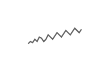
\begin{tikzpicture}[x=0.08em, y=0.08em, line width=0.4pt]
                \draw[FooterGray] (0,3) -- (1,4) -- (2,3.5) -- (3,5) -- (4,4) -- (5,6) -- (6,5.5) -- (7,4) -- (8,5) -- (9,7) -- (10,6) -- (11,5) -- (12,6.5) -- (13,8) -- (14,7) -- (15,6) -- (16,7.5) -- (17,9) -- (18,8) -- (19,7) -- (20,8.5) -- (21,10) -- (22,9) -- (23,8) -- (24,9.5);
            \end{tikzpicture}%
        }%
        \hskip0.5cm%
    }%
    \vskip6pt%
}

%=============================================================================
% PACHETE
%=============================================================================
\usepackage[utf8]{inputenc}
\usepackage[T1]{fontenc}
\usepackage{amsmath, amssymb, amsthm}
\usepackage{mathtools}
\usepackage{bm}
\usepackage{tikz}
\usetikzlibrary{arrows.meta, positioning, shapes, calc, decorations.pathreplacing, shadings}
\usepackage{booktabs}
\usepackage{multirow}
\usepackage{array}
\usepackage{graphicx}
\usepackage{hyperref}
\usepackage{colortbl}
\usepackage{pifont}
\hypersetup{colorlinks=true, linkcolor=MainBlue, urlcolor=MainBlue}
\graphicspath{{../../logos/}{../../charts/}{../../photos/}}
\hfuzz=3pt  % Suppress tiny overfull warnings (<3pt)
\vfuzz=2pt  % Suppress tiny vertical overfull warnings (<2pt)

%=============================================================================
% COMANDA QUANTLET
%=============================================================================
\newcommand{\quantlet}[2]{%
    \vspace{-0.25cm}%
    \hfill\href{#2}{%
        \raisebox{-0.15em}{
\includegraphics[height=0.7em]{ql_logo.png}}%
        \textcolor{MainBlue}{\tiny\ #1}%
    }\par%
}

%=============================================================================
% PAGINĂ TITLU PERSONALIZATĂ
%=============================================================================
\defbeamertemplate*{title page}{hybrid}[1][]
{
    \vspace{0.2cm}
    % Rând logo-uri - antet superior (cu linkuri clickabile)
    \begin{center}
        \href{https://www.ase.ro}{
\includegraphics[height=1.0cm]{ase_logo.png}}\hspace{0.3cm}%
        \href{https://theida.net}{
\includegraphics[height=1.0cm]{ida_logo.png}}\hspace{0.3cm}%
        \href{https://blockchain-research-center.com}{
\includegraphics[height=1.0cm]{brc_logo.png}}\hspace{0.3cm}%
        \href{https://www.ai4efin.ase.ro}{
\includegraphics[height=1.0cm]{ai4efin_logo.png}}\hspace{0.3cm}%
        \href{https://ipe.ro/new}{
\includegraphics[height=1.0cm]{acad_logo.png}}\hspace{0.3cm}%
        \href{https://www.digital-finance-msca.com}{
\includegraphics[height=1.0cm]{msca_logo.png}}%
    \end{center}

    \vspace{0.6cm}

    % Titlu principal cu logo-uri Q pe părți (cu linkuri clickabile)
    \begin{center}
        \begin{minipage}{0.1\textwidth}
            \centering
            \href{https://quantlet.com}{
\includegraphics[height=1.1cm]{ql_logo.png}}
        \end{minipage}%
        \begin{minipage}{0.78\textwidth}
            \centering
            {\LARGE\bfseries\usebeamercolor[fg]{title}\inserttitle}

            \vspace{0.3cm}

            {\usebeamerfont{subtitle}\usebeamercolor[fg]{title}\insertsubtitle}
        \end{minipage}%
        \begin{minipage}{0.1\textwidth}
            \centering
            \href{https://quantinar.com}{
\includegraphics[height=1.1cm]{qr_logo.png}}
        \end{minipage}
    \end{center}

    \vspace{0.6cm}

    % Autori (aliniere la stânga)
    \hspace{0.5cm}\begin{minipage}[t]{0.9\textwidth}
        \usebeamerfont{author}\insertauthor
    \end{minipage}

    \vspace{0.3cm}

    % Institut/Afilieri (aliniere la stânga)
    \hspace{0.5cm}\begin{minipage}[t]{0.9\textwidth}
        \raggedright\small\insertinstitute
    \end{minipage}
}

%=============================================================================
% MEDII PENTRU TEOREME
%=============================================================================
\theoremstyle{definition}
\setbeamertemplate{theorems}[numbered]
\newtheorem{defn}{Definiție}
\newtheorem{thm}{Teoremă}
\newtheorem{prop}{Propoziție}
\newtheorem{rmk}{Observație}

%=============================================================================
% CENTRED MINIPAGE
%=============================================================================
\newenvironment{cminipage}[1]{%
    \par\noindent\hfill\begin{minipage}{#1}\ignorespaces
}{%
    \end{minipage}\hfill\null\par
}

%=============================================================================
% COMENZI PERSONALIZATE
%=============================================================================
\newcommand{\E}{\mathbb{E}}
\newcommand{\Var}{\text{Var}}
\newcommand{\Cov}{\text{Cov}}
\newcommand{\Corr}{\text{Corr}}
\newcommand{\R}{\mathbb{R}}
\newcommand{\N}{\mathbb{N}}
\newcommand{\Z}{\mathbb{Z}}
\newcommand{\B}{\mathbf{B}}
\newcommand{\imark}{\textcolor{MainBlue}{\textbullet}}
\newcommand{\RMSE}{\text{RMSE}}
\newcommand{\MAE}{\text{MAE}}
\newcommand{\MAPE}{\text{MAPE}}

% Indicatoare nivel academic pe slide-uri  (numeric \ifnum — bulletproof in beamer templates)
\newcount\slidelevelnum
\global\slidelevelnum=0
\makeatletter
\newcommand{\slidelevel}[1]{%
    \global\slidelevelnum=0%
    \def\tmp@SL{#1}\def\tmp@SLy{Y3}\def\tmp@SLm{MSc}\def\tmp@SLp{PhD}%
    \ifx\tmp@SL\tmp@SLy \global\slidelevelnum=1\fi%
    \ifx\tmp@SL\tmp@SLm \global\slidelevelnum=2\fi%
    \ifx\tmp@SL\tmp@SLp \global\slidelevelnum=3\fi%
}
\makeatother
\gdef\currentlevelcolor{FooterGray}
\newcommand{\showlevel}{%
    \ifnum\slidelevelnum=1%
        \colorbox{Forest}{\strut\textcolor{white}{\sffamily\bfseries\fontsize{8}{9}\selectfont Y3}}%
        \gdef\currentlevelcolor{Forest}%
    \fi%
    \ifnum\slidelevelnum=2%
        \colorbox{MainBlue}{\strut\textcolor{white}{\sffamily\bfseries\fontsize{8}{9}\selectfont MSc}}%
        \gdef\currentlevelcolor{MainBlue}%
    \fi%
    \ifnum\slidelevelnum=3%
        \colorbox{Crimson}{\strut\textcolor{white}{\sffamily\bfseries\fontsize{8}{9}\selectfont PhD}}%
        \gdef\currentlevelcolor{Crimson}%
    \fi%
    \ifnum\slidelevelnum=0%
        \gdef\currentlevelcolor{FooterGray}%
    \fi%
}

%=============================================================================
% INFORMAȚII TITLU
%=============================================================================
\title[Statistica Piețelor Financiare]{Statistica Piețelor Financiare}
\subtitle{Capitolul 3: Distribuții stabile ($\alpha$-stabile)}
\author[D.T. Pele, A. Amza]{\texorpdfstring{\begin{tabular}[t]{@{}l@{}}Daniel Traian PELE \\ Antoaneta Amza\end{tabular}}{Daniel Traian PELE, Antoaneta Amza}}
\institute{Academia de Studii Economice din București\\
IDA Institute Digital Assets\\
Blockchain Research Center\\
AI4EFin Artificial Intelligence for Energy Finance\\
Academia Română, Institutul de Prognoză Economică\\
MSCA Digital Finance}
\date{}

\begin{document}

% Pagina de titlu (fără antet/subsol)
{
\setbeamertemplate{headline}{}
\setbeamertemplate{footline}{}
\begin{frame}
    \titlepage
\end{frame}
}

%=============================================================================
% GHID DE STUDIU
%=============================================================================
\begin{frame}{Ghid de studiu --- Cum să folosiți materialele}
\begin{columns}[T]
\begin{column}{0.48\textwidth}
\begin{block}{Înainte de curs (\textit{pre-reading})}
\begin{itemize}\setlength\itemsep{2pt}
\item Nolan (2020), Cap.\ 1 (20 pag.)
\item Mandelbrot (1963), primele 10 pag.
\item Opțional: Samorodnitsky \& Taqqu (1994), Cap.\ 1
\end{itemize}
\end{block}
\end{column}
\begin{column}{0.48\textwidth}
\begin{block}{După curs (\textit{review})}
\begin{itemize}\setlength\itemsep{2pt}
\item Refaceți exercițiile din slide-uri \textbf{fără} a privi rezolvările
\item Rulați notebook-ul Quantlet \texttt{SFM\_ch2\_stable\_distributions}
\item Completați testele grilă din seminar ca auto-evaluare
\end{itemize}
\end{block}
\end{column}
\end{columns}
\vspace{0.2cm}
\begin{alertblock}{Resurse digitale}
\begin{itemize}\setlength\itemsep{1pt}
\item \textbf{Slide-uri + cod}: \url{https://danpele.github.io/SFM/}
\item \textbf{Quantlet-uri interactive}: \url{https://github.com/QuantLet/Stat_fin_markets/tree/master/Ch_02}
\item \textbf{Forum de discuții}: Platforma e-learning ASE
\end{itemize}
\end{alertblock}
\end{frame}

%=============================================================================
% OBIECTIVE DE ÎNVĂȚARE
%=============================================================================
\begin{frame}{Obiective de învățare}
    \begin{block}{La sfârșitul acestui capitol, veți fi capabili să:}
    \begin{enumerate}
        \item[\textcolor{MainBlue}{\textbf{1.}}] \textbf{Definiți} distribuțiile $\alpha$-stabile și explicați cei patru parametri ($\alpha, \beta, \gamma, \delta$)
        \item[\textcolor{MainBlue}{\textbf{2.}}] \textbf{Enunțați} Teorema Limită Centrală Generalizată (TLCG) și rolul distribuțiilor stabile
        \item[\textcolor{MainBlue}{\textbf{3.}}] \textbf{Explicați} de ce varianța poate fi infinită ($\alpha < 2$) și implicațiile pentru teoria Markowitz
        \item[\textcolor{MainBlue}{\textbf{4.}}] \textbf{Estimați} parametrii stabili prin MLE și interpretați rezultatele
        \item[\textcolor{MainBlue}{\textbf{5.}}] \textbf{Comparați} distribuțiile stabile cu Normala și Student-$t$ (cozi, momente, proprietăți)
        \item[\textcolor{MainBlue}{\textbf{6.}}] \textbf{Descrieți} procesele L\'{e}vy stabile și distribuțiile stabile temperate
    \end{enumerate}
    \end{block}
\end{frame}

%=============================================================================
% CUPRINS
%=============================================================================
{
\setbeamertemplate{headline}{%
    \vskip10pt%
    \hbox to \paperwidth{\hskip0.5cm\hfill\hskip0.5cm}%
    \vskip4pt%
    {\color{FooterGray}\hrule height 0.4pt}%
}
\begin{frame}{}
    {\color{FooterGray}\hrule height 0.4pt}
    \vspace{0.1cm}
    {\Large\textcolor{IDAred}{\textbf{Cuprins}}}
    \vspace{0.2cm}
    {\small
    \begin{columns}[T]
        \begin{column}{0.48\textwidth}
            \begin{itemize}
                \item Definiție și parametri
                \item Varianța infinită
                \item Ajustare pe date financiare
                \item Funcția caracteristică
                \item TLCG
            \end{itemize}
        \end{column}
        \begin{column}{0.48\textwidth}
            \begin{itemize}
                \item Estimare și analiză cross-asset
                \item Stabilă vs.\ Student-$t$
                \item Procese L\'{e}vy
                \item Stabile temperate
                \item Anexă: Aprofundare
            \end{itemize}
        \end{column}
    \end{columns}
    }
\end{frame}
}

%=============================================================================
% SECȚIUNEA 1: DISTRIBUȚII STABILE
%=============================================================================
\section{Distribuții stabile ($\alpha$-stabile)}

%--- Y3 Slide 1 ---
\slidelevel{Y3}
\begin{frame}{Ce este o distribuție stabilă?}
\begin{defn}[Distribuție stabilă --- Intuitiv]
O distribuție este \textbf{stabilă} dacă suma de copii i.i.d.\ are aceeași formă (până la locație și scală). Formal, $X \sim S(\alpha, \beta, \gamma, \delta)$ dacă pentru copii i.i.d.\ $X_1, X_2$:
\[
aX_1 + bX_2 \stackrel{d}{=} cX + d, \quad c = (a^\alpha + b^\alpha)^{1/\alpha}.
\]
\end{defn}

\begin{itemize}
\item \textbf{Patru parametri}:
\begin{itemize}
\item $\alpha \in (0, 2]$: \textbf{indicele de stabilitate} (grosimea cozilor) --- $\alpha$ mai mic $\Rightarrow$ cozi mai groase
\item $\beta \in [-1, 1]$: \textbf{asimetrie}
\item $\gamma > 0$: \textbf{scală}
\item $\delta \in \R$: \textbf{locație}
\end{itemize}
\item Cazuri speciale: $\alpha = 2$ (Gaussiană), $\alpha = 1, \beta = 0$ (Cauchy)
\end{itemize}
\end{frame}

%--- Y3 Slide 1b ---
\slidelevel{Y3}
\begin{frame}{Densitățile $\alpha$-stabile --- Efectul lui $\alpha$}
\vspace{-0.2cm}
\begin{center}
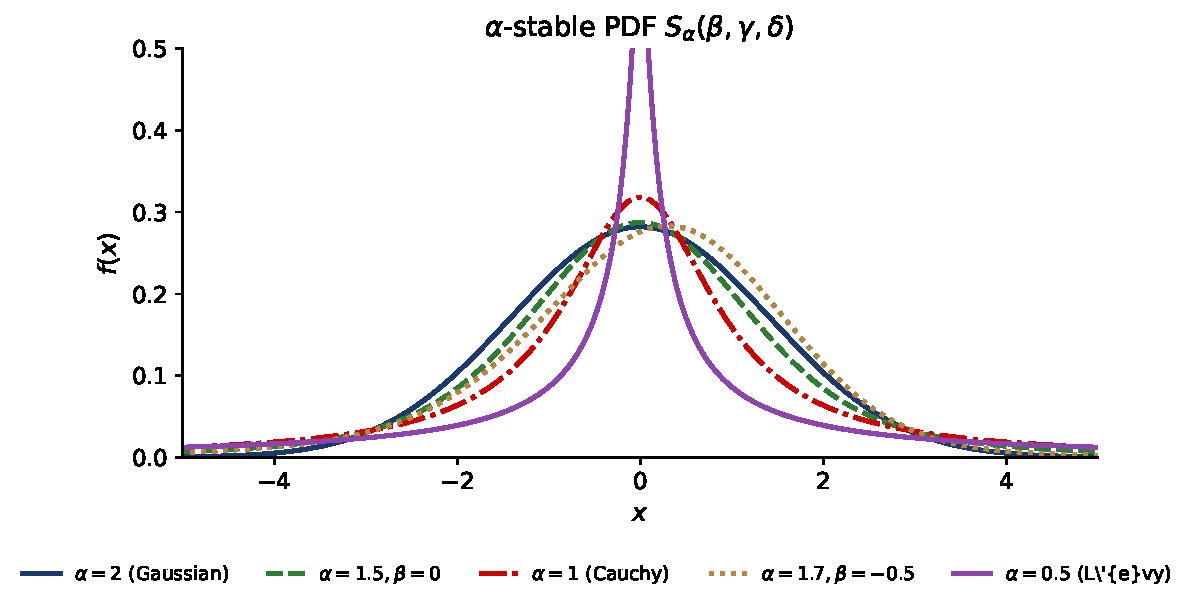
\includegraphics[width=0.52\textwidth]{ch2_stable_pdf_theoretical.pdf}
\end{center}
\vspace{-0.2cm}
\begin{itemize}
\item $\alpha = 2$: \textbf{Gaussiană}; \quad $\alpha < 2$: cozi \textbf{lege putere} $f(x) \sim |x|^{-(1+\alpha)}$
\item $\alpha = 1$: \textbf{Cauchy} ($\E[|X|] = \infty$); \quad $\beta \neq 0$: introduce \textbf{asimetrie}
\end{itemize}
\end{frame}

%--- Y3 Slide 2 ---
\slidelevel{Y3}
\begin{frame}{De ce varianța poate să nu existe}
\begin{itemize}
\item Pentru $\alpha < 2$: $\E[|X|^p] < \infty$ dacă și numai dacă $p < \alpha$
\item În particular, $\E[X^2] = \infty$ când $\alpha < 2$ --- \textbf{varianța nu există}
\item Varianța eșantionului nu converge la o constantă; crește odată cu $n$
\item \textbf{Mandelbrot (1963)}: variațiile prețului bumbacului urmează legi stabile cu $\alpha \approx 1{,}7$
\item Estimări tipice pentru randamente financiare: $\hat{\alpha} \in [1{,}5;\ 1{,}9]$
\end{itemize}
\end{frame}

%--- Y3 Slide 2b ---
\slidelevel{Y3}
\begin{frame}{Varianța eșantionului --- convergență vs.\ divergență}
\vspace{-0.1cm}
\begin{center}
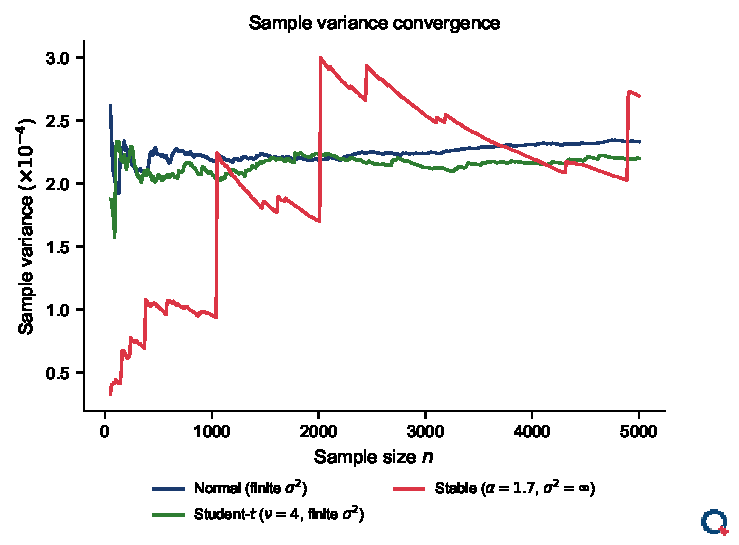
\includegraphics[width=0.4\textwidth]{ch2_sample_var_diverge.pdf}
\end{center}
\quantlet{SFM\_ch2\_stable\_distributions}{https://github.com/QuantLet/Stat_fin_markets/tree/master/Ch_02/SFM_ch2_stable_distributions}
\vspace{-0.3cm}
\begin{alertblock}{Schimbare de paradigmă}
\begin{itemize}
\item Dacă $\alpha < 2$, teoria medie-varianță (Markowitz) se prăbușește: varianța nu este o măsură semnificativă de risc
\end{itemize}
\end{alertblock}
\end{frame}

%--- Y3 Slide 3 ---
\slidelevel{Y3}
\begin{frame}{Ajustarea stabilă pe S\&P 500}
\begin{center}
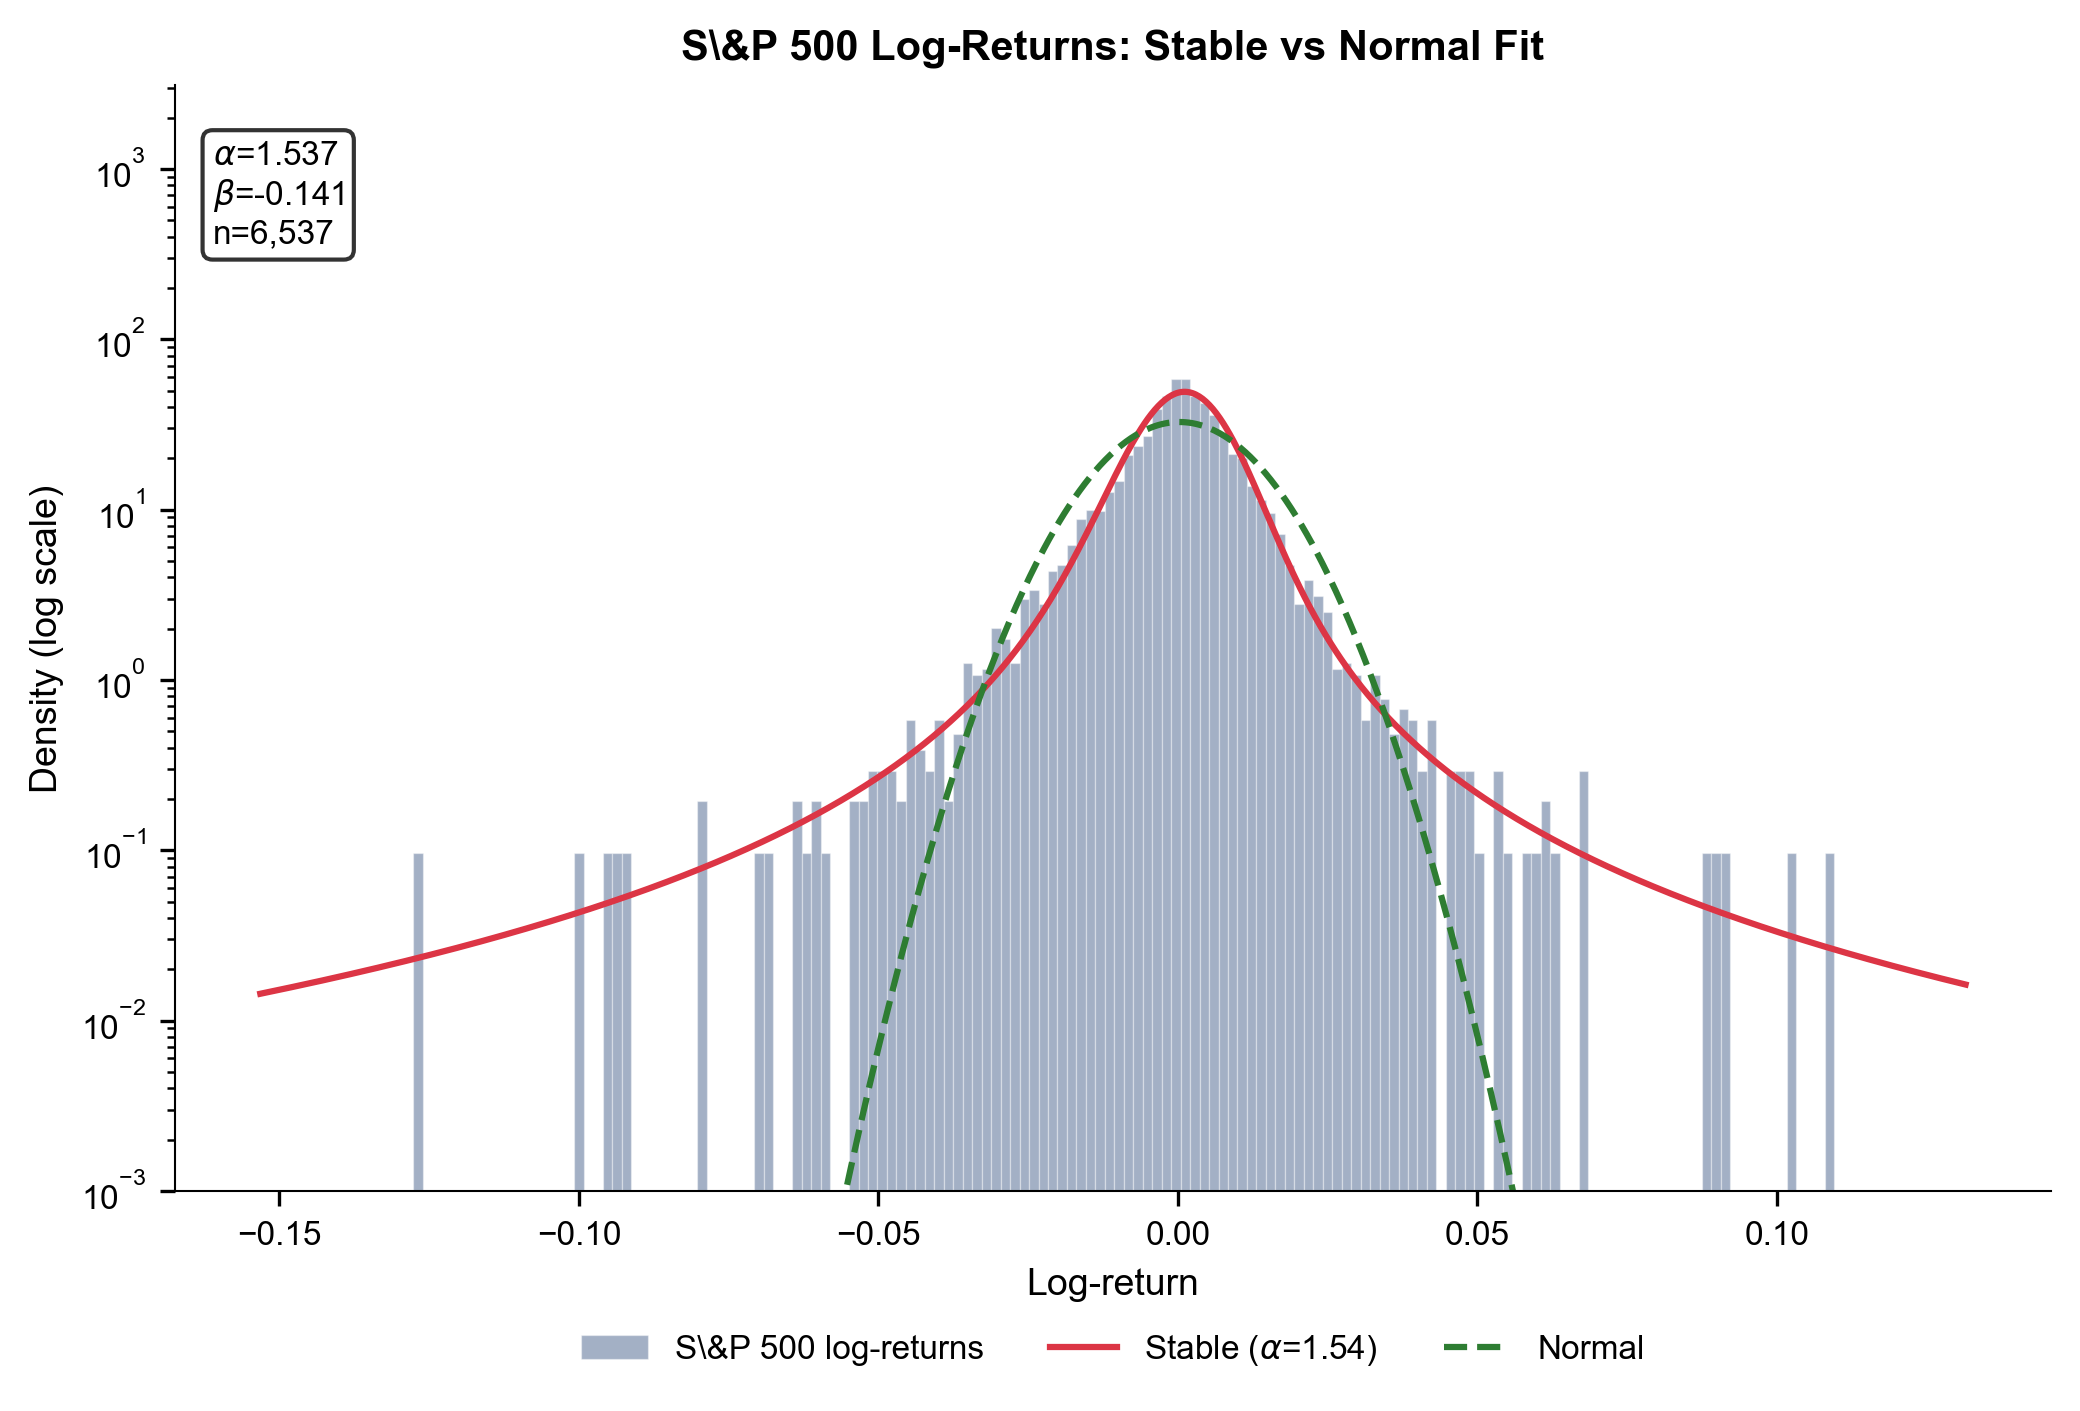
\includegraphics[width=0.5\textwidth]{ch2_sp500_stable_fit.png}
\end{center}
\quantlet{SFM\_ch2\_stable\_distributions}{https://github.com/QuantLet/Stat_fin_markets/tree/master/Ch_02/SFM_ch2_stable_distributions}

\begin{itemize}
\item Distribuția stabilă surprinde cozile groase mai bine decât distribuția normală
\item $\hat{\alpha} \approx 1{,}7$ estimat pentru randamentele zilnice S\&P~500
\end{itemize}
\end{frame}

%--- Y3 Slide 4 ---
\slidelevel{Y3}
\begin{frame}{Stabilă vs.\ Normală vs.\ Student-$t$}
\begin{center}
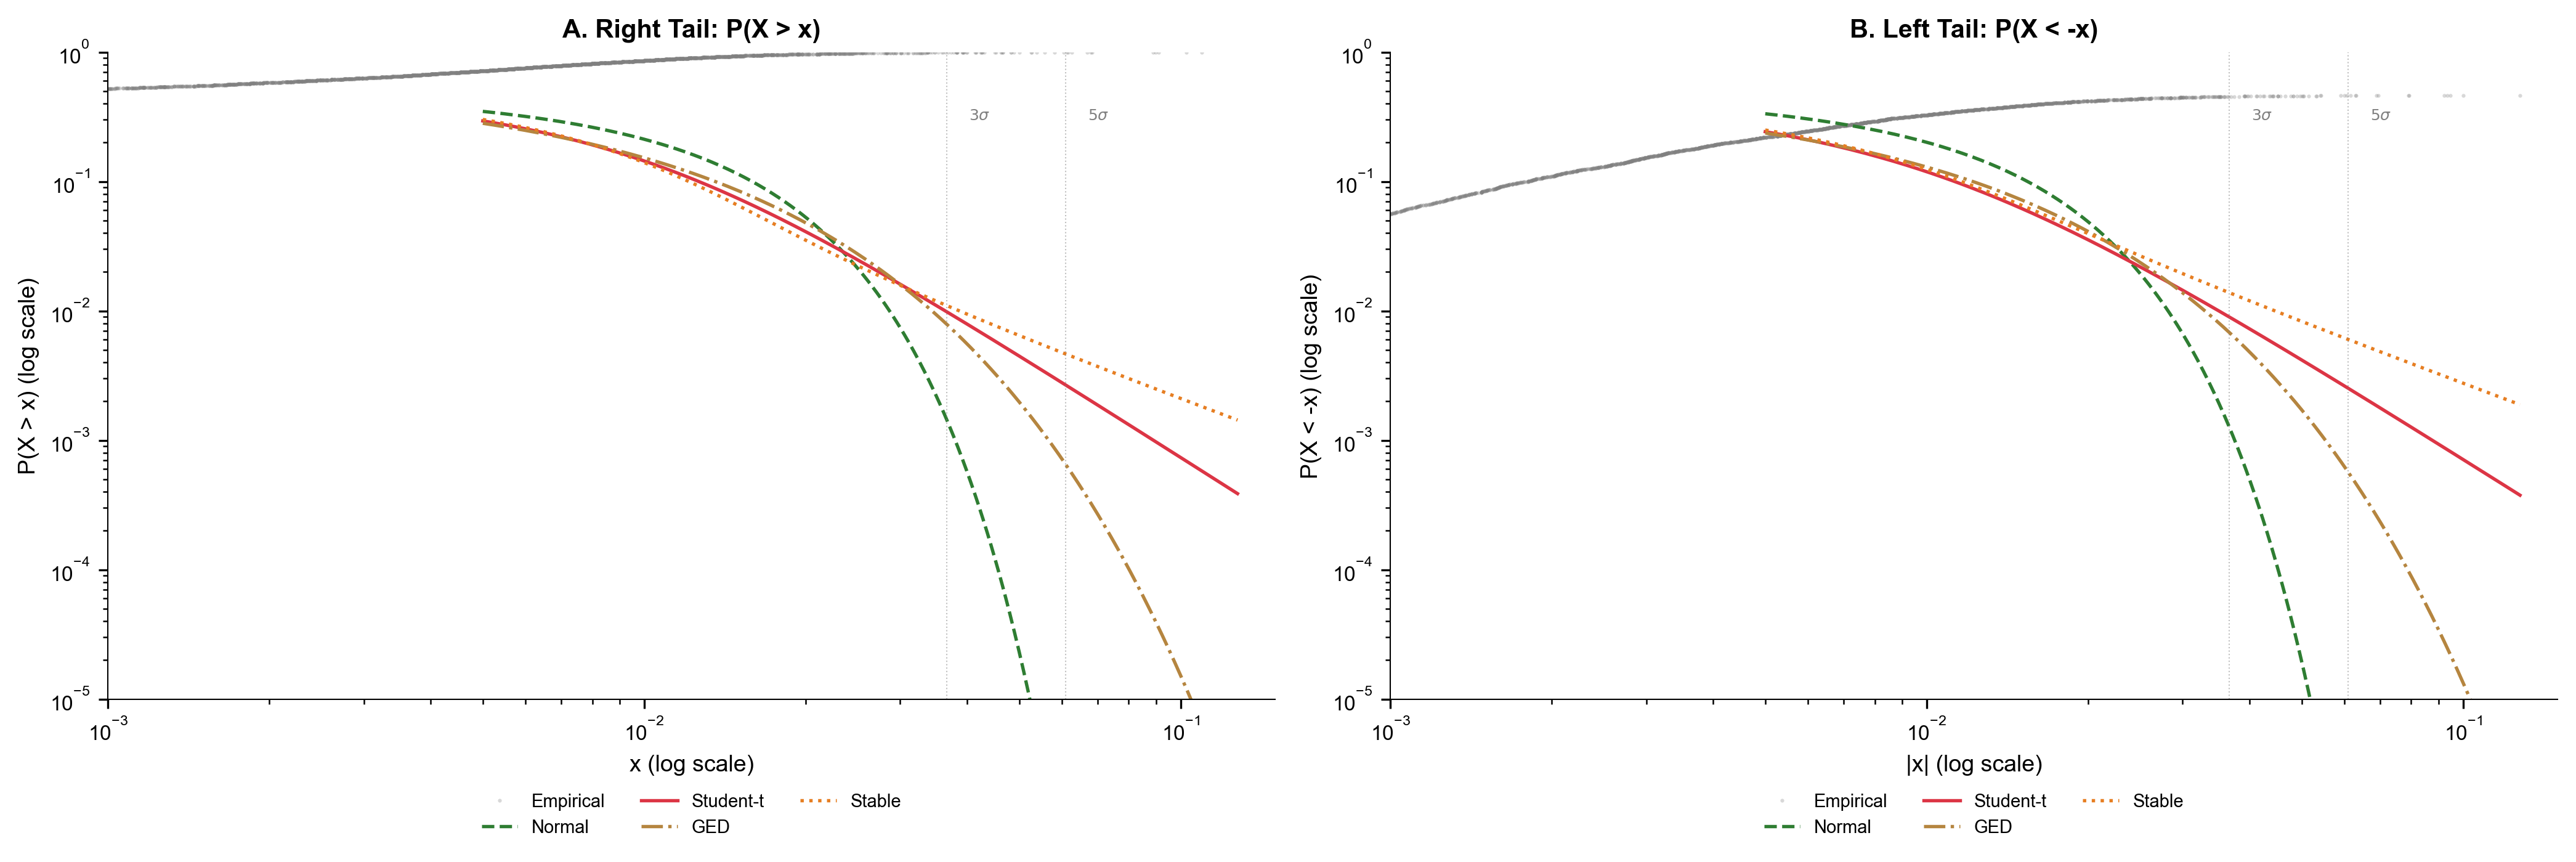
\includegraphics[width=0.65\textwidth]{ch2_dist_comparison_tails.png}
\end{center}
\quantlet{SFM\_ch2\_stable\_distributions}{https://github.com/QuantLet/Stat_fin_markets/tree/master/Ch_02/SFM_ch2_stable_distributions}
\begin{center}
\renewcommand{\arraystretch}{1.1}
\begin{tabular}{lccc}
\toprule
& \textbf{Normală} & \textbf{Student-$t$} & \textbf{Stabilă} \\
\midrule
Descreșterea cozii (PDF) & $e^{-x^2/2}$ & $|x|^{-\nu-1}$ & $|x|^{-\alpha-1}$ \\
Varianța & Finită & Finită ($\nu>2$) & Infinită ($\alpha<2$) \\
Închisă la sumă & Da & Nu & Da \\
Limită TLC & TLC & --- & TLCG \\
\bottomrule
\end{tabular}
\end{center}
\end{frame}

%--- MSc Slide 5 ---
\slidelevel{MSc}
\begin{frame}{Funcția caracteristică}
\begin{itemize}
\item Distribuția stabilă este definită prin \textbf{funcția caracteristică} (parametrizarea Nolan $S^1$, $\alpha \neq 1$):
\end{itemize}
\[
\phi(t) = \E[e^{itX}] = \exp\!\left\{-\gamma^\alpha |t|^\alpha\!\left(1 - i\beta\,\text{sign}(t)\tan\frac{\pi\alpha}{2}\right) + i\delta t\right\}
\]
\begin{itemize}
\item Cazul $\alpha = 1$:
\end{itemize}
\[
\phi(t) = \exp\!\left\{-\gamma|t|\!\left(1 + i\beta\frac{2}{\pi}\,\text{sign}(t)\ln|t|\right) + i\delta t\right\}
\]

\begin{itemize}
\item \textbf{Fără PDF în formă închisă} în general (excepții: Gaussiană, Cauchy, L\'{e}vy)
\item Densitatea prin transformata Fourier inversă: $f(x) = \frac{1}{2\pi}\int_{-\infty}^{\infty}\phi(t)\,e^{-itx}\,dt$
\item Evaluare numerică: algoritmul lui Nolan (1997)
\end{itemize}
\begin{rmk}
\begin{itemize}
\item Utilizăm parametrizarea $S^1(\alpha,\beta,\gamma,\delta)$ a lui Nolan (1997) în tot capitolul
\item \texttt{scipy.stats.levy\_stable} folosește parametrizarea $S^0$ --- atenție la conversie!
\end{itemize}
\end{rmk}
\end{frame}

%--- MSc Slide 6 ---
\slidelevel{MSc}
\begin{frame}{Teorema Limită Centrală Generalizată}
\begin{thm}[TLCG]
Distribuțiile stabile sunt singurele limite non-degenerate posibile ale sumelor normalizate:
\[
\frac{S_n - b_n}{a_n} \xrightarrow{d} S(\alpha, \beta, \gamma, \delta)
\]
unde $S_n = X_1 + \cdots + X_n$ pentru $X_i$ i.i.d.
\end{thm}

\begin{itemize}
\item TLC clasică: $\alpha = 2$ (necesită varianță finită)
\item TLCG: $\alpha < 2$ (permite varianță infinită)
\item \textbf{Proprietatea de stabilitate}: Sumele de v.a.\ stabile i.i.d.\ rămân stabile cu același $\alpha$
\item \textbf{Cozi tip lege putere}: $P(X > x) \sim C_\alpha(1+\beta)\,x^{-\alpha}$ când $x \to \infty$
\end{itemize}
\end{frame}

%--- MSc Slide 7 ---
\slidelevel{MSc}
\begin{frame}{PDF-uri stabile --- Variind $\alpha$}
\begin{center}
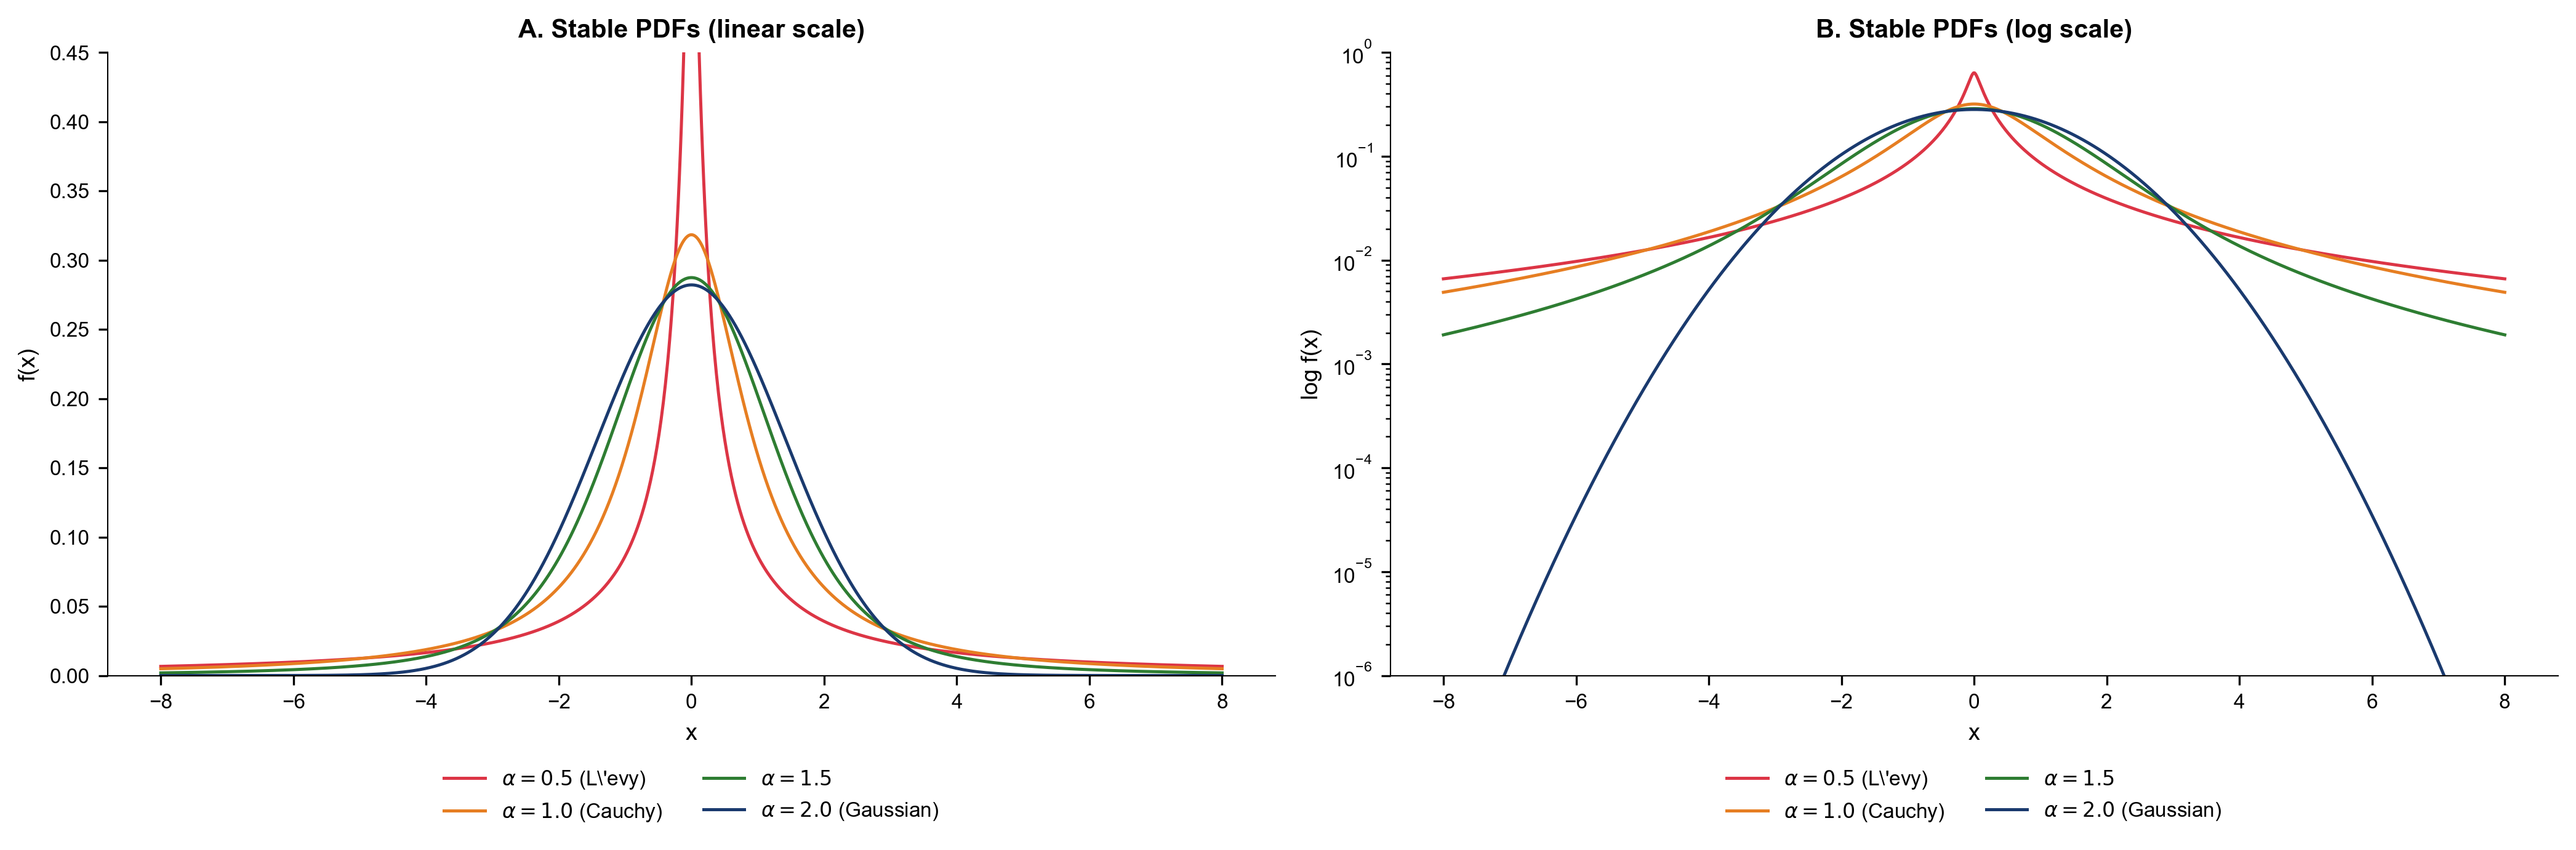
\includegraphics[width=0.72\textwidth]{ch2_stable_pdfs.png}
\end{center}
\quantlet{SFM\_ch2\_stable\_distributions}{https://github.com/QuantLet/Stat_fin_markets/tree/master/Ch_02/SFM_ch2_stable_distributions}
\begin{itemize}
\item $\alpha$ mai mic $\Rightarrow$ cozi mai groase, vârf mai ascuțit
\item $\alpha = 2$: Gaussiană; $\alpha = 1$: Cauchy
\item Randamente financiare: $\hat{\alpha} \in [1{,}5;\ 1{,}9]$
\end{itemize}
\end{frame}

%--- MSc Slide 8 ---
\slidelevel{MSc}
\begin{frame}{Estimare și analiză cross-asset}
\begin{columns}[T]
\begin{column}{0.48\textwidth}
\begin{block}{Metode de estimare}
\begin{itemize}
\item Metoda cuantilelor McCulloch (rapidă, consistentă)
\item MLE (Nolan, 1997) --- cea mai eficientă
\item Metode bazate pe funcția caracteristică (Kogon \& Williams, 1998)
\end{itemize}
\end{block}
\end{column}
\begin{column}{0.48\textwidth}
\begin{center}
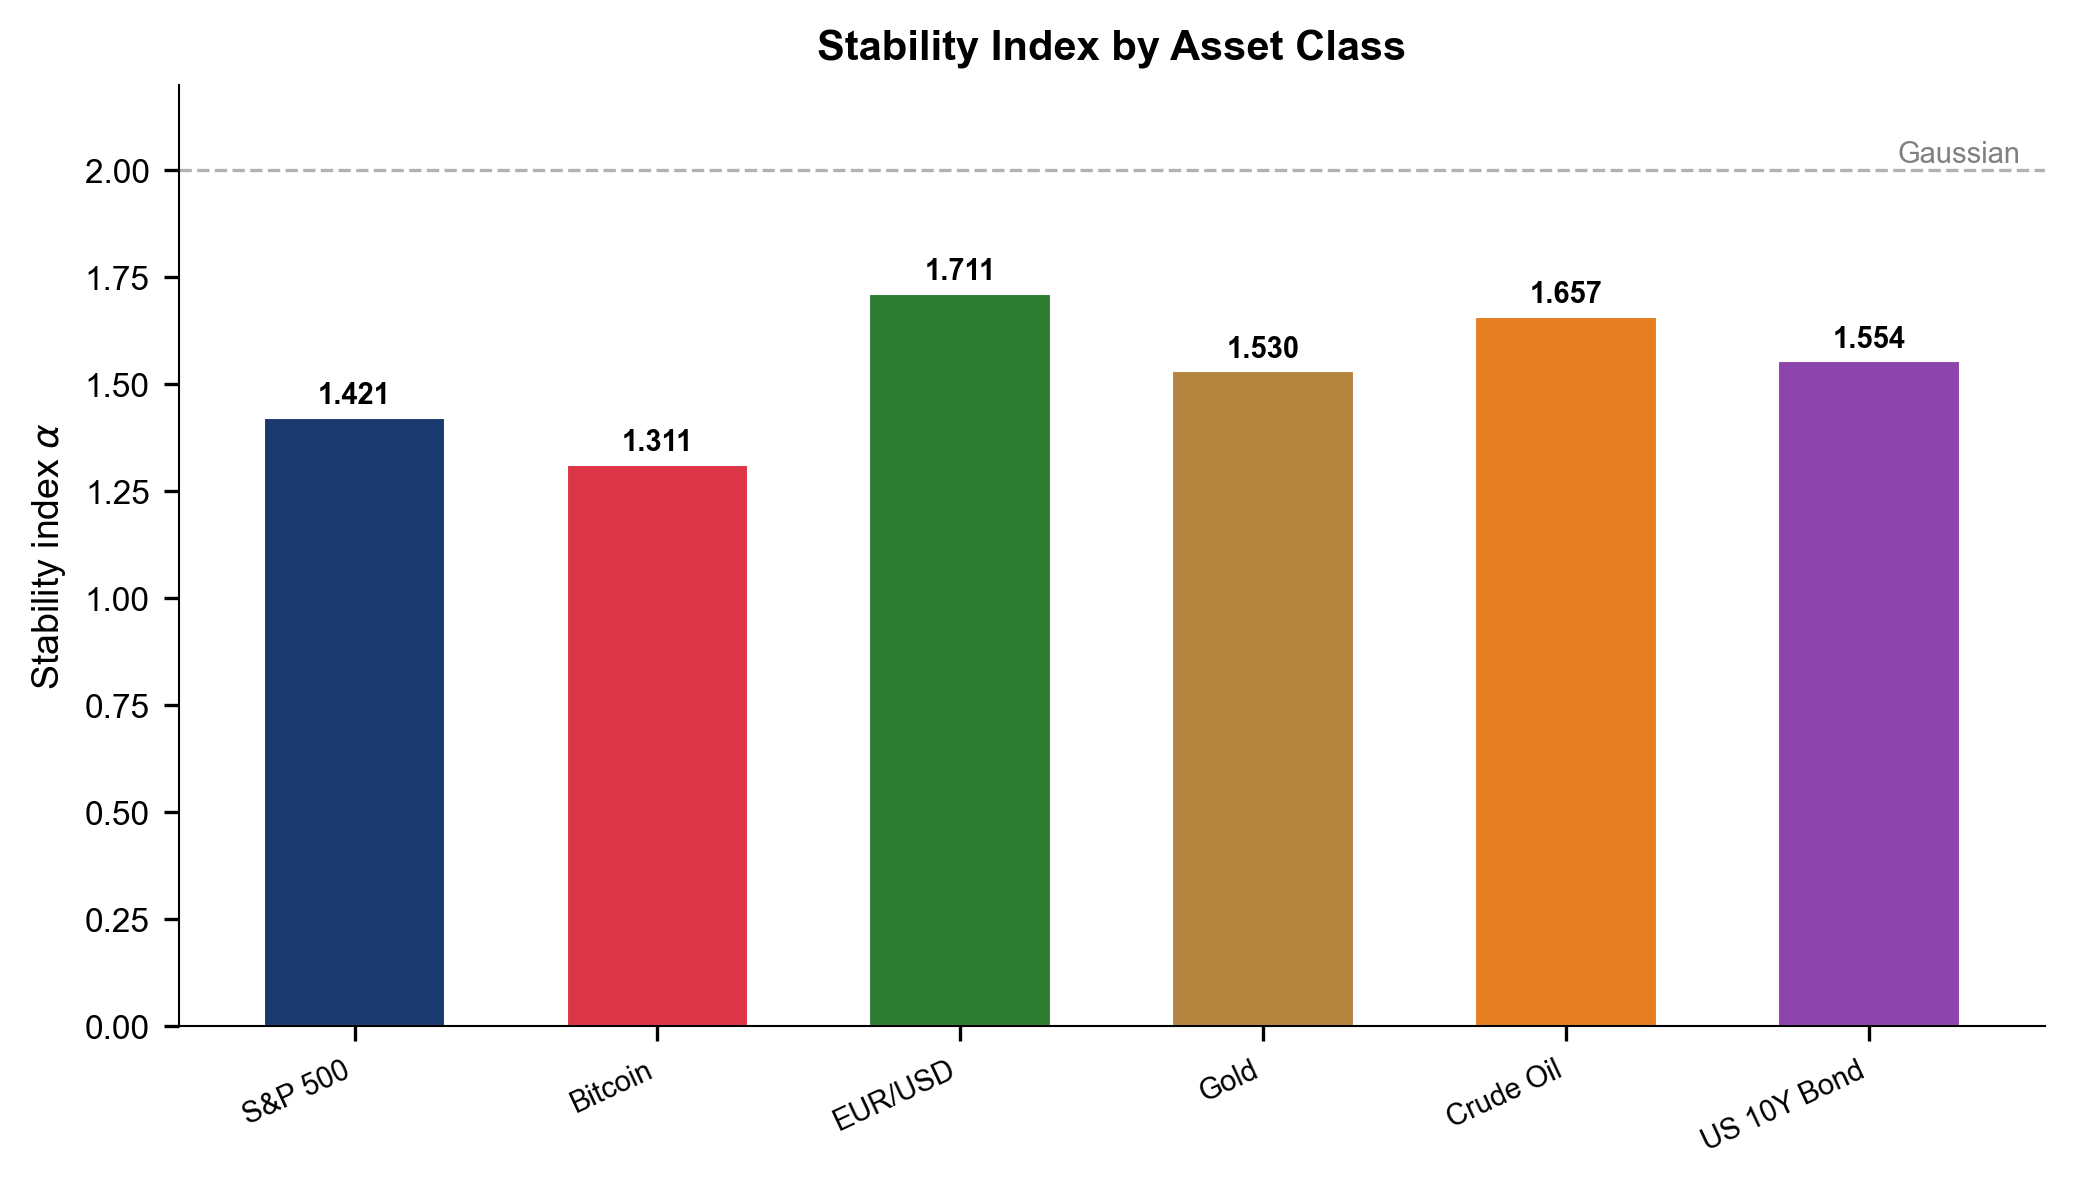
\includegraphics[width=\textwidth]{ch2_cross_asset_alpha.png}
\end{center}
\quantlet{SFM\_ch2\_stable\_distributions}{https://github.com/QuantLet/Stat_fin_markets/tree/master/Ch_02/SFM_ch2_stable_distributions}
\end{column}
\end{columns}

\vspace{0.2cm}
\begin{itemize}
\item $\hat{\alpha} \approx 1{,}7$ pentru S\&P~500; $\hat{\alpha} \approx 1{,}5$ pentru Bitcoin; $\hat{\alpha} \approx 1{,}8$ pentru FX
\item $\alpha < 2$ pentru toate clasele majore de active $\Rightarrow$ varianța infinită este ubicuă
\end{itemize}
\end{frame}

%--- PhD Slide 8b ---
\slidelevel{PhD}
\begin{frame}{$\alpha_{\text{stabil}}$ vs.\ $\alpha_{\text{Hill}}$ --- Reconciliere}
\begin{columns}[T]
\begin{column}{0.48\textwidth}
\begin{block}{MLE pe toată distribuția}
\begin{itemize}
\item $\hat{\alpha}_{\text{stabil}} \approx 1{,}7$ (S\&P~500)
\item Captează \textbf{comportamentul global}
\item Include centrul + cozile
\item Implică varianță infinită ($\alpha < 2$)
\end{itemize}
\end{block}
\end{column}
\begin{column}{0.48\textwidth}
\begin{block}{Estimatorul Hill (doar coada)}
\begin{itemize}
\item $\hat{\alpha}_{\text{Hill}} \approx 3\text{--}4$ (S\&P~500)
\item Estimează doar \textbf{indexul de coadă}
\item Folosește doar observațiile extreme
\item Implică varianță finită ($\alpha > 2$)
\end{itemize}
\end{block}
\end{column}
\end{columns}

\vspace{0.1cm}
\begin{alertblock}{Reconciliere: distribuții stabile temperate}
\begin{itemize}
\item Conflictul $\hat{\alpha}_{\text{stabil}} \neq \hat{\alpha}_{\text{Hill}}$ este \textbf{aparent}: cele două estimează cantități diferite
\item Distribuțiile \textbf{stabile temperate} (CGMY) rezolvă paradoxul: comportament stabil pentru $x$ moderat, dar cozi cu decădere exponențial-multiplicată
\item Referințe: McCulloch (1997), Grabchak \& Samorodnitsky (2010)
\end{itemize}
\end{alertblock}
\end{frame}

%--- PhD Slide 9 ---
\slidelevel{PhD}
\begin{frame}{Variație regulată și domeniu de atracție}
\begin{defn}[Variație regulată]
$L : (0,\infty) \to (0,\infty)$ este \textbf{lent variabilă} la infinit dacă $\lim_{x\to\infty} L(tx)/L(x) = 1$ pentru orice $t > 0$. O funcție $f$ este \textbf{regulat variabilă} cu indice $\rho$ dacă $f(x) = x^\rho L(x)$.
\end{defn}

\begin{thm}[Domeniul de atracție]
$F$ aparține domeniului de atracție al $S(\alpha, \beta, 1, 0)$ dacă și numai dacă:
\begin{enumerate}
\item $\bar{F}(x) = x^{-\alpha}L(x)$ (cozi regulat variabile)
\item Condiția de echilibru: $\lim_{x\to\infty} \frac{\bar{F}(x)}{\bar{F}(x) + F(-x)} = \frac{1+\beta}{2}$
\end{enumerate}
\end{thm}

\vspace{0.1cm}
{\small\textit{Variația regulată fundamentează teoria EVT și determină dacă estimatorul Hill este consistent.}}
\end{frame}


%--- PhD Slide 10 ---
\slidelevel{PhD}
\begin{frame}{Procese L\'{e}vy}
\begin{itemize}
\item Un \textbf{proces L\'{e}vy} $\{L_t\}_{t\geq 0}$ are creșteri staționare independente
\item $L_1 \sim S(\alpha, \beta, \gamma, \delta)$ definește un \textbf{proces L\'{e}vy stabil}
\item \textbf{Descompunerea L\'{e}vy--It\^{o}}:
\[
L_t = bt + \sigma W_t + \int_{|x|\leq 1} x\,\tilde{N}(t,dx) + \int_{|x|>1} x\,N(t,dx)
\]
\item \textbf{Măsura L\'{e}vy} a unui proces stabil:
\[
\nu(dx) = \begin{cases} c_+ x^{-\alpha-1}dx & x > 0 \\ c_- |x|^{-\alpha-1}dx & x < 0 \end{cases}
\]
\item Activitate infinită: infinit de multe salturi mici în orice interval finit
\end{itemize}

\begin{rmk}[De ce contează?]
\begin{itemize}
\item Procesele Lévy sunt fundamentul evaluării opțiunilor cu salturi; Black--Scholes $= \nu \equiv 0$
\item Componenta de salt explică zâmbetul volatilității
\end{itemize}
\end{rmk}
\end{frame}

%--- PhD Slide 11 ---
\slidelevel{PhD}
\begin{frame}{Distribuții stabile temperate}
\begin{itemize}
\item \textbf{Problemă}: Distribuțiile stabile pure au varianță infinită --- incomod pentru unele aplicații
\item \textbf{Soluție}: Distribuții stabile temperate --- modificăm măsura L\'{e}vy:
\[
\nu(dx) = c\,|x|^{-\alpha-1}e^{-\lambda|x|}dx
\]
\item Păstrează comportamentul de coadă grea pentru $x$ moderat dar garantează \textbf{momente finite}
\item Temperarea exponențială elimină coada extremă $\Rightarrow$ toate momentele există
\end{itemize}
\end{frame}


%--- PhD Slide 12 ---
\slidelevel{PhD}
\begin{frame}{Stabilă vs.\ Student-$t$: Marea dezbatere}
\begin{center}
\renewcommand{\arraystretch}{1.0}
\footnotesize
\begin{tabular}{lcc}
\toprule
& \textbf{Stabilă} & \textbf{Student-$t$} \\
\midrule
Indice de coadă & $\alpha$ & $\nu$ \\
Momente finite & $p < \alpha$ & $p < \nu$ \\
Închisă la sumă & Da & Nu \\
Limită TLCG & Da & Nu \\
Varianța & $\infty$ ($\alpha < 2$) & Finită ($\nu > 2$) \\
Estimare & Mai dificilă (fără PDF) & MLE standard \\
\bottomrule
\end{tabular}
\end{center}
\begin{itemize}
\item Dezbatere istorică: Mandelbrot--Fama (stabile) vs.\ Praetz--Blattberg--Gonedes (Student-$t$)
\item Viziunea modernă: ambele surprind cozi tip lege putere; alegerea depinde de aplicație
\end{itemize}
\begin{center}
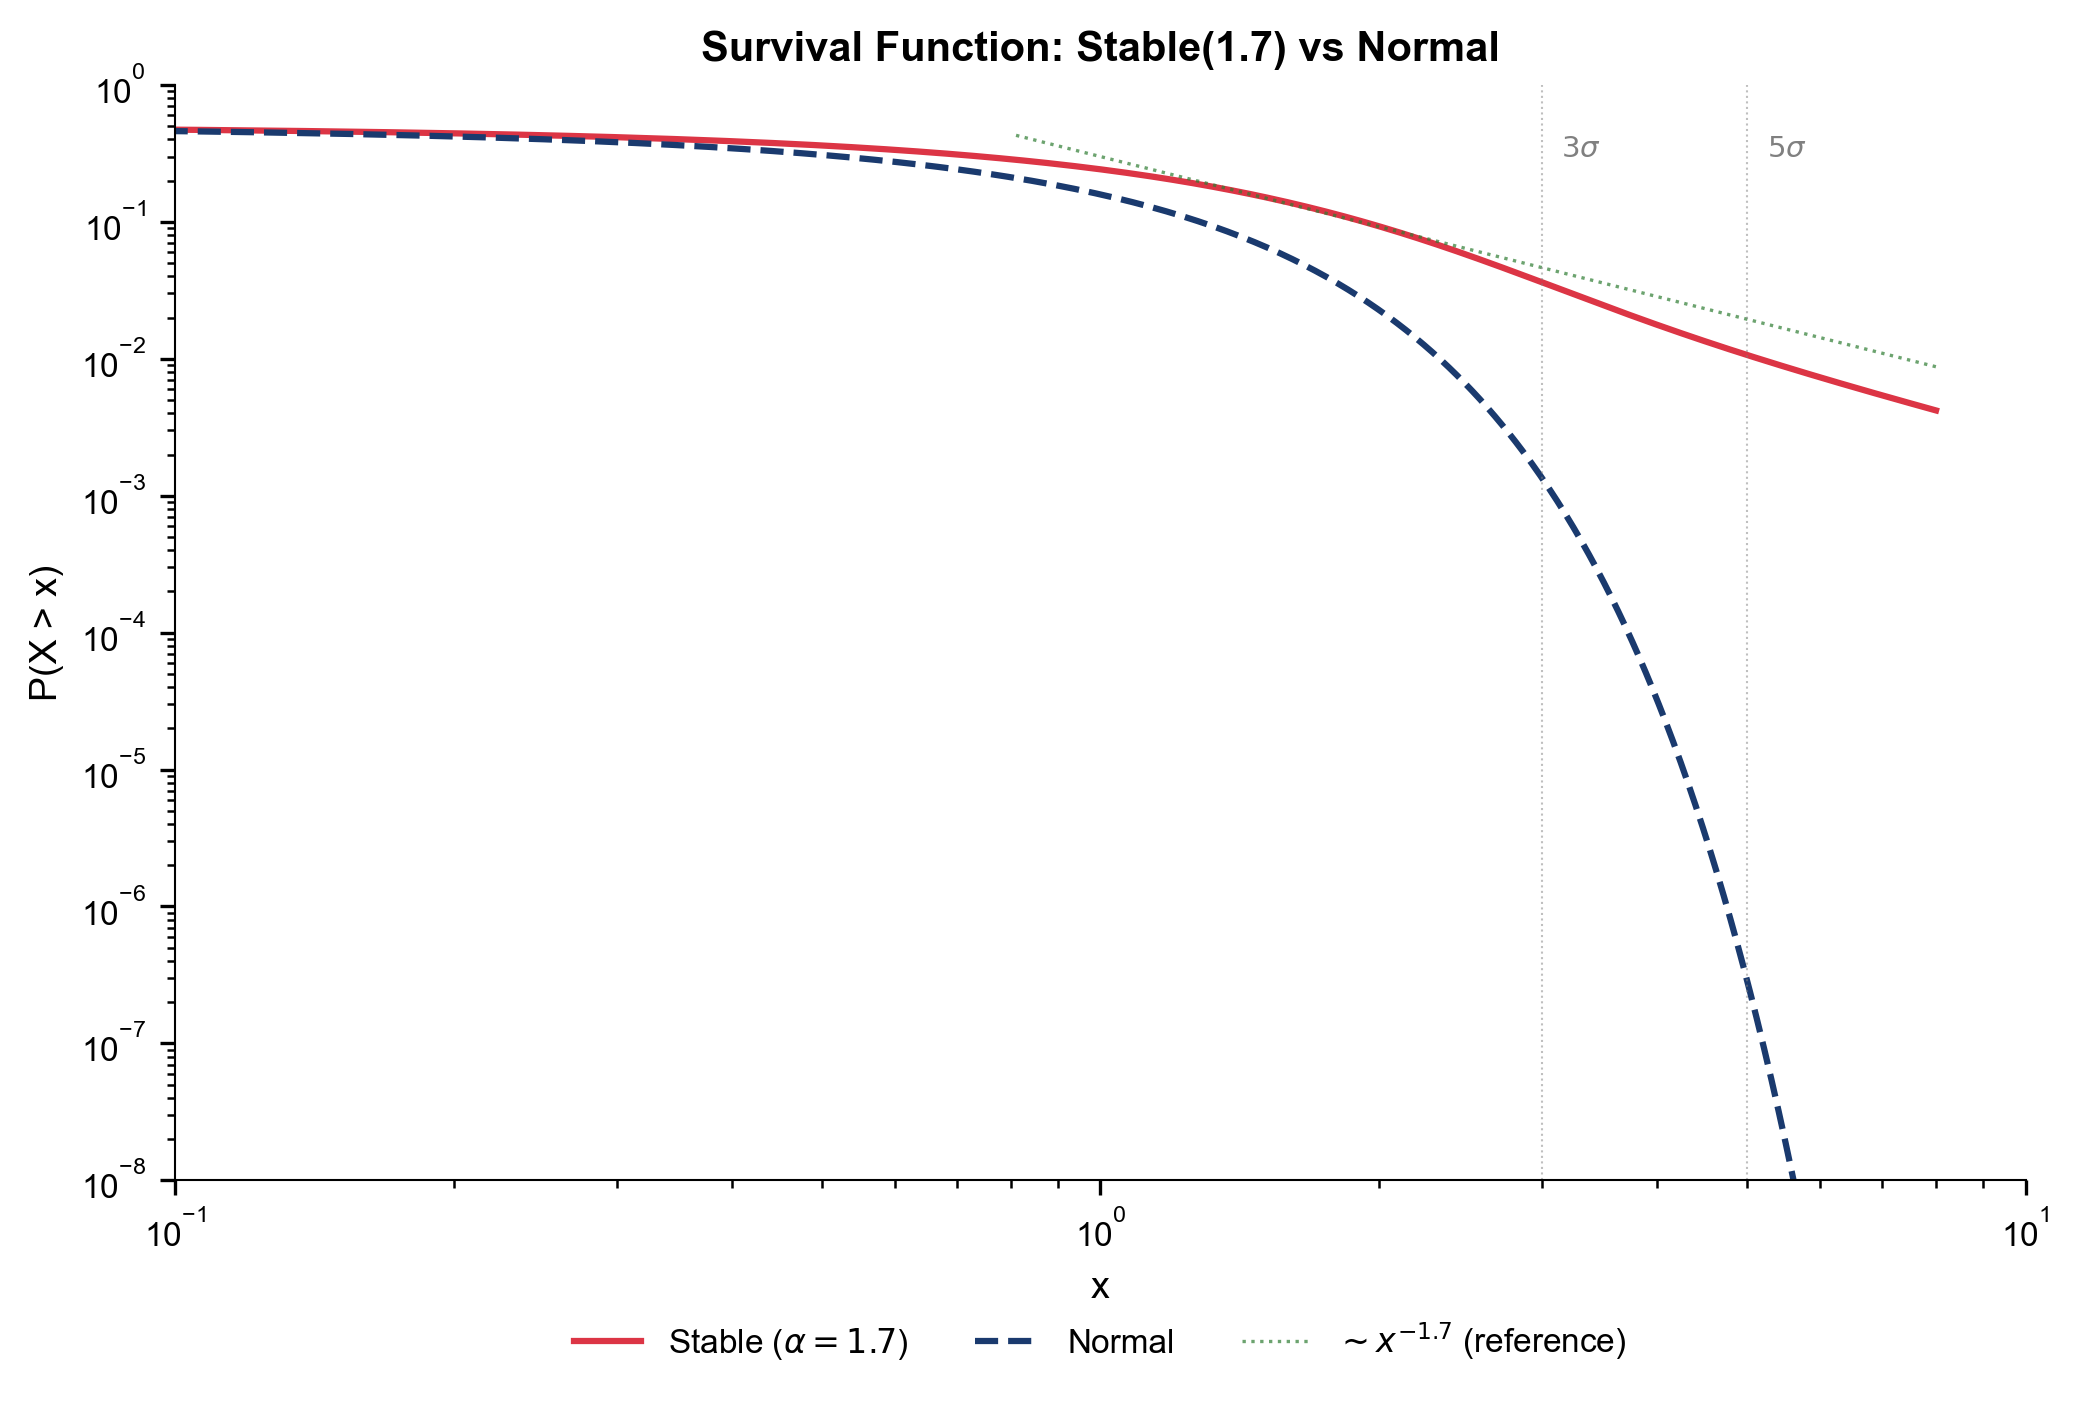
\includegraphics[width=0.25\textwidth]{ch2_tail_survival.png}
\end{center}
\quantlet{SFM\_ch2\_stable\_distributions}{https://github.com/QuantLet/Stat_fin_markets/tree/master/Ch_02/SFM_ch2_stable_distributions}
\end{frame}

%--- Y3 Slide 13 ---
\slidelevel{Y3}
\begin{frame}{Exemplu: Interpretarea parametrilor stabili}
\begin{exampleblock}{Exercițiu: MLE pe S\&P~500 (2000--2023)}
$\hat{\alpha} = 1{,}70$, $\hat{\beta} = -0{,}10$, $\hat{\gamma} = 0{,}0058$, $\hat{\delta} = 0{,}0003$. Interpretați parametrii.
\end{exampleblock}

\begin{block}{Interpretare}
\begin{itemize}
\item $\hat{\alpha} = 1{,}70 < 2$: \textbf{varianță infinită} --- cozile descresc ca $|x|^{-1{,}70}$, mai lent decât $e^{-x^2/2}$
\item $\hat{\beta} = -0{,}10 < 0$: ușoară \textbf{asimetrie la stânga} --- coada pierdere mai grea
\item $\hat{\gamma} = 0{,}0058$: parametru de \textbf{scală} (analog $\sigma$, dar $\sigma^2 = \infty$)
\item $\hat{\delta} = 0{,}0003$: \textbf{locația} (randamentul mediu zilnic $\approx 0{,}03\%$)
\end{itemize}
\end{block}

\begin{alertblock}{Consecință}
\begin{itemize}
\item Dacă $\alpha = 1{,}70$, $P(|r| > 5\hat{\gamma})$ este de $\sim$12$\times$ mai mare decât sub distribuția normală
\item Markowitz medie-varianță \textbf{nu este validă}
\end{itemize}
\end{alertblock}
\end{frame}

%=============================================================================
% QUICK CHECK --- Distribuții stabile
%=============================================================================
\begin{frame}{Opriți-vă și gândiți-vă \hfill {\normalsize\textcolor{MediumGray}{\textit{(auto-evaluare)}}}}
\begin{alertblock}{Verificare rapidă --- Distribuții stabile}
\begin{enumerate}\setlength\itemsep{4pt}
\item O distribuție stabilă cu $\alpha = 1{,}7$ are varianță finită? Dar medie?
\item Mandelbrot a propus distribuții stabile pentru randamente. Dacă $\alpha < 2$, ce implicație are pentru teoria lui Markowitz (medie-varianță)?
\item Pe S\&P~500, $\hat{\alpha} \approx 1{,}7$. Probabilitatea $P(|r| > 5\hat{\gamma})$ este de $\sim$12$\times$ mai mare decât sub normală. Ce înseamnă aceasta practic?
\end{enumerate}
\end{alertblock}
\vspace{0.1cm}
\begin{exampleblock}{Răspunsuri}
\begin{enumerate}\setlength\itemsep{0pt}
\item Varianță: \textbf{nu} ($\alpha < 2$ $\Rightarrow$ varianță infinită). Medie: \textbf{da} ($\alpha > 1$).
\item Markowitz \textbf{nu este valid}: necesită varianță finită. Trebuie optimizare bazată pe alte măsuri de risc (CVaR, spectral).
\item Evenimentele extreme (crize) sunt mult mai frecvente decât prezice modelul Gaussian --- capitalul regulamentar trebuie ajustat.
\end{enumerate}
\end{exampleblock}
\end{frame}

%=============================================================================
% QUIZ
%=============================================================================
\section{Quiz}

\slidelevel{Y3}
\begin{frame}{Întrebarea 1}
    \begin{cminipage}{0.95\textwidth}
    \begin{alertblock}{Întrebare}
        \begin{itemize}
            \item Care proprietate face distribuțiile $\alpha$-stabile unice din punct de vedere teoretic?
        \end{itemize}
    \end{alertblock}

    \vspace{0.3cm}

    \begin{block}{Variante de răspuns}

        \textcolor{MainBlue}{\textbf{(A)}} Au cozi exponențiale (scad rapid)\\[3pt]

        \textcolor{MainBlue}{\textbf{(B)}} Sunt singurele limite posibile ale sumelor normalizate (TLCG)\\[3pt]

        \textcolor{MainBlue}{\textbf{(C)}} Au întotdeauna varianță finită\\[3pt]

        \textcolor{MainBlue}{\textbf{(D)}} Sunt întotdeauna simetrice

    \end{block}
    \end{cminipage}
\end{frame}

\slidelevel{Y3}
\begin{frame}{Întrebarea 1: Răspuns}
    \begin{cminipage}{0.95\textwidth}
    \begin{exampleblock}{Răspuns: (B)}
    \begin{itemize}
        \item Teorema Limită Centrală Generalizată (TLCG) arată că distribuțiile stabile sunt \textbf{singurele} limite posibile ale sumelor normalizate de v.a.\ i.i.d.
        \item (A) este invers: distribuțiile stabile cu $\alpha < 2$ au cozi \textbf{groase} (lege putere), nu exponențiale.
        \item (C) este greșit: pentru $\alpha < 2$, varianța este infinită.
        \item (D) este greșit: parametrul $\beta \in [-1,1]$ controlează asimetria.
    \end{itemize}
    \end{exampleblock}
    \end{cminipage}
\end{frame}

\slidelevel{Y3}
\begin{frame}{Întrebarea 2}
    \begin{cminipage}{0.95\textwidth}
    \begin{alertblock}{Întrebare}
        \begin{itemize}
            \item Un portofoliu de \$10M are VaR zilnic la 1\% de: \$230k (normală), \$380k (Student-$t$, $\nu=5$), \$520k (stabilă, $\alpha=1{,}7$). Ce concluzie trageți?
        \end{itemize}
    \end{alertblock}

    \vspace{0.3cm}

    \begin{block}{Variante de răspuns}

        \textcolor{MainBlue}{\textbf{(A)}} Distribuția normală este cea mai conservatoare\\[3pt]

        \textcolor{MainBlue}{\textbf{(B)}} Alegerea distribuției nu afectează semnificativ VaR\\[3pt]

        \textcolor{MainBlue}{\textbf{(C)}} Subestimarea riscului de coadă sub ipoteza normală poate fi de $2\times$ sau mai mult\\[3pt]

        \textcolor{MainBlue}{\textbf{(D)}} Distribuția stabilă subestimează întotdeauna riscul

    \end{block}
    \end{cminipage}
\end{frame}

\slidelevel{Y3}
\begin{frame}{Întrebarea 2: Răspuns}
    \begin{cminipage}{0.95\textwidth}
    \begin{exampleblock}{Răspuns: (C)}
    \begin{itemize}
        \item VaR normală = \$230k, VaR stabilă = \$520k $\Rightarrow$ raportul este $520/230 \approx 2{,}3\times$.
        \item Distribuția normală \textbf{subestimează} riscul, nu este conservatoare (elimină A).
        \item Diferența de \$290k ($= 520 - 230$) este \textbf{foarte semnificativă} din perspectiva capitalului (elimină B).
        \item Aceasta demonstrează de ce Basel~III impune modele cu cozi groase.
    \end{itemize}
    \end{exampleblock}
    \end{cminipage}
\end{frame}

%=============================================================================
% EXERCIȚII DE EXAMEN
%=============================================================================
\section{Exerciții de examen}

\slidelevel{MSc}
\begin{frame}{Exercițiul 1: Distribuții stabile}
\begin{block}{Enunț}
Un cercetător ajustează o distribuție stabilă pe randamentele Bitcoin și obține $(\hat{\alpha}, \hat{\beta}, \hat{\gamma}, \hat{\delta}) = (1{,}72;\; -0{,}15;\; 0{,}008;\; 0{,}001)$.
\end{block}
\begin{enumerate}
    \item Interpretați fiecare parametru economic: ce spun $\alpha$, $\beta$, $\gamma$, $\delta$?
    \item Această distribuție are varianță finită? Justificați.
    \item Cum se compară cozile cu cele ale distribuției normale?
    \item Ce implică $\beta = -0{,}15$ pentru asimetria riscului?
\end{enumerate}
\vspace{0.1cm}
\begin{exampleblock}{De reținut}
$\alpha \in (0,2]$: indice de stabilitate (greutatea cozilor); $\beta \in [-1,1]$: asimetrie; $\gamma > 0$: scală; $\delta$: locație. Varianța finită doar dacă $\alpha = 2$.
\end{exampleblock}
\end{frame}

%=============================================================================
% REZOLVĂRI EXERCIȚII
%=============================================================================
\section*{Rezolvări exerciții}

\slidelevel{MSc}
\begin{frame}{Exercițiul 1: Rezolvare}
\begin{block}{Rezolvare}
Date: $(\hat{\alpha}, \hat{\beta}, \hat{\gamma}, \hat{\delta}) = (1{,}72,\; -0{,}15,\; 0{,}008,\; 0{,}001)$.

\textbf{1.} Interpretare:
\begin{itemize}
\item $\alpha = 1{,}72$: cozi groase (mai groase decât distribuția normală, $\alpha = 2$); mai aproape de Cauchy ($\alpha=1$)
\item $\beta = -0{,}15$: asimetrie negativă (coada stângă mai grea $\Rightarrow$ pierderi extreme mai probabile)
\item $\gamma = 0{,}008$: parametru de scală (similar deviației standard)
\item $\delta = 0{,}001$: locație (aproape de zero, randament mediu zilnic)
\end{itemize}

\textbf{2.} $\alpha = 1{,}72 < 2$ $\Rightarrow$ varianță \textbf{infinită}. Doar momentele de ordin $p < 1{,}72$ sunt finite.

\textbf{3.} Cozile scad ca $|x|^{-1{,}72-1} = |x|^{-2{,}72}$ vs.\ $e^{-x^2/2}$ (normală). Mult mai lent $\Rightarrow$ evenimente extreme mult mai probabile.

\textbf{4.} $\beta < 0$: coada stângă este mai grea decât coada dreaptă $\Rightarrow$ riscul de pierdere este asimetric.
\end{block}
\end{frame}

%=============================================================================
% LABORATOR PYTHON
%=============================================================================
\slidelevel{MSc}
\begin{frame}{Laborator Python --- Distribuții stabile}
\small
\begin{exampleblock}{Lab: Estimare și comparație}
Rulați \texttt{SFM\_ch2\_stable\_distributions.ipynb}:
\begin{enumerate}
\item Estimați $(\hat{\alpha}, \hat{\beta}, \hat{\gamma}, \hat{\delta})$ pe randamente S\&P~500
\item Grafic PDF stabilă vs.\ normală vs.\ Student-$t$
\item Calculați VaR 1\% sub toate cele trei modele. Raportați diferențele
\end{enumerate}
\end{exampleblock}
\quantlet{SFM\_ch2\_stable\_distributions}{https://github.com/QuantLet/Stat_fin_markets/tree/master/Ch_02/SFM_ch2_stable_distributions}

\vspace{0.3cm}
\begin{block}{Teme pentru acasă}
\begin{enumerate}
\item Descărcați date zilnice pentru o acțiune. Ajustați distribuția stabilă prin MLE. Raportați $(\hat{\alpha}, \hat{\beta}, \hat{\gamma}, \hat{\delta})$.
\item Comparați graficul QQ sub distribuția normală, Student-$t$ și stabilă. Care model surprinde cel mai bine cozile?
\item Calculați VaR 1\% sub fiecare model. Raportați diferențele procentuale.
\end{enumerate}
\end{block}
\end{frame}

%=============================================================================
% ANEXĂ: APROFUNDARE --- DISTRIBUȚII STABILE (PhD)
%=============================================================================

\section*{Anexă: Aprofundare --- Distribuții stabile}

%--- PhD Slide A1 ---
\slidelevel{PhD}
\begin{frame}{Anexă: Variație regulată de ordin secund}
\begin{defn}[Variație regulată de ordin secund]
O funcție de supraviețuire $\bar{F}$ satisface condiția de variație regulată de ordin secund dacă:
\[
\bar{F}(x) = x^{-\alpha}L(x)\left(1 + \frac{b}{\rho}x^{\rho} + o(x^{\rho})\right), \quad x \to \infty
\]
unde $\rho < 0$ este \textbf{parametrul de ordin secund} și $b \neq 0$.
\end{defn}

\begin{itemize}
\item $\rho$ controlează \textbf{rata de convergență} către comportamentul asimptotic tip lege putere
\item $|\rho|$ mic $\Rightarrow$ convergență lentă $\Rightarrow$ bias mare al estimatorului Hill
\item $|\rho|$ mare $\Rightarrow$ convergență rapidă $\Rightarrow$ estimatorul Hill este fiabil cu mai puține date extreme
\item Bias-ul estimatorului Hill: $\text{Bias}(\hat{\alpha}_H) \approx \frac{b}{\rho(\alpha-\rho)} k^{-\rho/\alpha} n^{\rho/\alpha}$
\item Alegerea optimală a $k$ depinde de $\rho$ --- Referințe: Hall (1982), de Haan \& Stadtmüller (1996)
\end{itemize}
\end{frame}

%--- PhD Slide A2 ---
\slidelevel{PhD}
\begin{frame}{Anexă: Modelul CGMY și evaluarea opțiunilor}
\begin{defn}[Procesul CGMY (Carr, Geman, Madan, Yor, 2002)]
Măsura Lévy:
\[
\nu(dx) = C\frac{e^{-G|x|}}{|x|^{1+Y}}\mathbf{1}_{x<0}\,dx + C\frac{e^{-Mx}}{x^{1+Y}}\mathbf{1}_{x>0}\,dx
\]
Funcția caracteristică:
\[
\ln\phi(u) = C\,\Gamma(-Y)\!\left[(M-iu)^Y - M^Y + (G+iu)^Y - G^Y\right]
\]
\end{defn}

\begin{itemize}
\item $C > 0$: intensitatea salturilor; $G, M > 0$: tempering; $Y \in (-\infty, 2)$: activitatea salturilor
\item $G \neq M$ $\Rightarrow$ asimetrie; $Y > 0$ $\Rightarrow$ activitate infinită; momente finite + cozi groase
\item Prețul opțiunii: $C(K) = \frac{e^{-rT}}{2\pi}\int e^{-iuK}\frac{\phi_T(u)}{u^2}\,du$ (Carr \& Madan, 1999)
\item CGMY explică zâmbetul volatilității fără a recurge la volatilitate stochastică
\end{itemize}
\end{frame}

%=============================================================================
% CRITERII DE EVALUARE
%=============================================================================
\begin{frame}{Criterii de evaluare --- Exerciții și proiect}
\begin{block}{Grila de notare (aplicabilă la examen și proiect)}
\small
\renewcommand{\arraystretch}{1.2}
\begin{center}
\begin{tabular}{lll}
\toprule
\textbf{Nivel} & \textbf{Calcul} & \textbf{Interpretare} \\
\midrule
\textcolor{Forest}{\textbf{9--10}} & Formule + calcule corecte, complete & Leagă de decizia de business \\
\textcolor{Amber}{\textbf{7--8}} & Formule corecte, erori minore & Interpretare corectă, superficială \\
\textcolor{Orange}{\textbf{5--6}} & Formula corectă, greșeli de aplicare & Repetă definiția fără context \\
\textcolor{Crimson}{\textbf{$<$5}} & Formula greșită sau lipsă & Fără interpretare \\
\bottomrule
\end{tabular}
\end{center}
\end{block}
\begin{alertblock}{Pondere evaluare}
\begin{itemize}\setlength\itemsep{0pt}
\item Examen scris: 70\% \quad Proiect individual: 20\% \quad Participare activă: 10\%
\end{itemize}
\end{alertblock}
\end{frame}

%=============================================================================
% LECTURĂ PE NIVELE
%=============================================================================
\begin{frame}{Lectură recomandată pe nivele}
\begin{block}{\textcolor{Forest}{\textbf{Y3}} --- Lectură minimă}
\begin{itemize}\setlength\itemsep{0pt}
\item Nolan (2020), Cap.\ 1.1--1.3 (definiție, parametri, cazuri speciale); exercițiul din curs
\end{itemize}
\end{block}
\begin{block}{\textcolor{MainBlue}{\textbf{MSc}} --- Lectură suplimentară}
\begin{itemize}\setlength\itemsep{0pt}
\item + Nolan (2020), Cap.\ 1--2 complet; Mandelbrot (1963); estimare MLE și comparație cross-asset
\end{itemize}
\end{block}
\begin{block}{\textcolor{Crimson}{\textbf{PhD}} --- Lectură avansată}
\begin{itemize}\setlength\itemsep{0pt}
\item + Samorodnitsky \& Taqqu (1994), Cap.\ 1--2; procese L\'{e}vy; CGMY; slide-urile Anexă
\end{itemize}
\end{block}
\end{frame}

%=============================================================================
% EXIT TICKET
%=============================================================================
\begin{frame}{Bilet de ieșire (\textit{Exit Ticket}) \hfill {\normalsize\textcolor{MediumGray}{\textit{(1 minut)}}}}
\begin{alertblock}{Completați înainte de a pleca (anonim, pe hârtie sau online)}
\begin{enumerate}\setlength\itemsep{6pt}
\item \textbf{Un lucru clar}: Ce concept din cursul de azi ați înțeles cel mai bine?
\item \textbf{Un lucru neclar}: Ce concept necesită mai multă clarificare?
\item \textbf{O întrebare}: Ce întrebare ați dori să explorați mai departe?
\end{enumerate}
\end{alertblock}
\vspace{0.3cm}
\begin{block}{De ce facem acest exercițiu?}
\begin{itemize}\setlength\itemsep{2pt}
\item Răspunsurile anonime ajustează conținutul \textbf{următorului curs}
\item Cercetările arată că reflecția imediat după curs crește retenția cu 20--40\% (Roediger \& Butler, 2011)
\end{itemize}
\end{block}
\end{frame}

%=============================================================================
% SECȚIUNEA: BIBLIOGRAFIE
%=============================================================================
\section{Bibliografie}

\begin{frame}{Bibliografie I}
    \begin{cminipage}{0.95\textwidth}
    \begin{block}{Manuale de referință}
        {\small
        \begin{itemize}\setlength{\itemsep}{0pt}
            \item Nolan, J. P. (2020). \textit{Stable Distributions --- Models for Heavy Tailed Data}. Birkh\"{a}user.
            \item Samorodnitsky, G. \& Taqqu, M. S. (1994). \textit{Stable Non-Gaussian Random Processes}. Chapman \& Hall.
            \item Rachev, S. T. (2003). \textit{Handbook of Heavy Tailed Distributions in Finance}. Elsevier.
        \end{itemize}
        }
    \end{block}

    \begin{exampleblock}{Articole fundamentale}
        {\small
        \begin{itemize}\setlength{\itemsep}{0pt}
            \item Mandelbrot, B. (1963). The Variation of Certain Speculative Prices. \textit{Journal of Business}, 36(4), 394--419.
            \item Fama, E. (1965). The Behavior of Stock-Market Prices. \textit{Journal of Business}, 38(1), 34--105.
            \item Nolan, J. P. (1997). Numerical Calculation of Stable Densities and Distribution Functions. \textit{Stochastic Models}, 13(4), 759--774.
        \end{itemize}
        }
    \end{exampleblock}
    \end{cminipage}
\end{frame}

\begin{frame}{Bibliografie II}
    \begin{cminipage}{0.95\textwidth}
    \begin{block}{Estimare și aplicații}
        {\small
        \begin{itemize}\setlength{\itemsep}{0pt}
            \item McCulloch, J. H. (1986). Simple Consistent Estimators of Stable Distribution Parameters. \textit{Comm.\ in Statistics --- Simulation and Computation}, 15(4), 1109--1136.
            \item Carr, P., Geman, H., Madan, D. B. \& Yor, M. (2002). The Fine Structure of Asset Returns. \textit{Journal of Business}, 75(2), 305--332.
            \item Grabchak, M. \& Samorodnitsky, G. (2010). Do Financial Returns Have Finite or Infinite Variance? \textit{Journal of Applied Probability}, 47(1), 103--118.
        \end{itemize}
        }
    \end{block}

    \begin{exampleblock}{Resurse online și cod}
        {\small
        \begin{itemize}\setlength{\itemsep}{0pt}
            \item \textbf{Quantlet}: \url{https://quantlet.com} $\succ$ Platformă de cod pentru metode cantitative
            \item \textbf{Quantinar}: \url{https://quantinar.com} $\succ$ Platformă de învățare pentru metode cantitative
            \item \textbf{GitHub SFM}: \url{https://github.com/QuantLet/Stat_fin_markets/tree/master/Ch_02} $\succ$ Cod Python
        \end{itemize}
        }
    \end{exampleblock}
    \end{cminipage}
\end{frame}

\begin{frame}{}
    \begin{cminipage}{0.95\textwidth}
        \centering
        \vspace{1cm}

        \Huge\textcolor{MainBlue}{Vă Mulțumim!}

        \vspace{0.8cm}

        \Large Întrebări?

        \vspace{1cm}

        \normalsize
        Materialele cursului sunt disponibile la: \url{https://danpele.github.io/SFM/}

        \vspace{0.3cm}

        \href{https://quantlet.com}{\raisebox{-0.15em}{
\includegraphics[height=0.8em]{ql_logo.png}} Quantlet} \hspace{0.5cm}
        \href{https://quantinar.com}{\raisebox{-0.15em}{
\includegraphics[height=0.8em]{qr_logo.png}} Quantinar}
    \end{cminipage}
\end{frame}
\end{document}
